\documentclass[a4paper,11pt,oneside]{jsbook}    %bookスタイルでないとchapterが使えないのでこのようにしている

%\usepackage{listings}
\usepackage[dvipdfmx]{graphicx}
\usepackage{setspace}
\usepackage{amsmath}
\usepackage{geometry}
\usepackage{here}
\usepackage{caption}
\usepackage{subcaption}
\usepackage{multirow}

% 参考文献リストで使用、使わない場合はコメントアウトしてもいい
\usepackage[numbers]{natbib}
% 添削時に意見をほしいなーって部分で使用した
\usepackage{color}


%%%%%%%%%%%%%%%%%%%%%%%%%%%%%%%%%%%%%%%%%%%%%%%%%%%%%%%%%%%%%%%%%%%%%%%%%
%%% 本文の行数と桁数を指定できるようにする
%%%%%%%%%%%%%%%%%%%%%%%%%%%%%%%%%%%%%%%%%%%%%%%%%%%%%%%%%%%%%%%%%%%%%%%%%
   \makeatletter
   \def\mojiparline#1{
        \newcounter{mpl}
        \setcounter{mpl}{#1}
        \@tempdima=\linewidth
        \advance\@tempdima by-\value{mpl}zw
        \addtocounter{mpl}{-1}
        \divide\@tempdima by \value{mpl}
        \advance\kanjiskip by\@tempdima
        \advance\parindent by\@tempdima
   }
   \makeatother
   \def\linesparpage#1{
       \baselineskip=\textheight
       \divide\baselineskip by #1
   }

\setstretch{0.5} % ページ全体の行間を設定

%%%%%%%%%%%%%%%%%%%%%%%%%%%%%%%%%%%%%%%%%%%%%%%%%%%%%%%%%%%%%%%%%%%%%%%%%
%%% ここからは個人的にほしいなー思ったコマンドの作成
%%%%%%%%%%%%%%%%%%%%%%%%%%%%%%%%%%%%%%%%%%%%%%%%%%%%%%%%%%%%%%%%%%%%%%%%%

%%% 数式で使用
\newcommand{\V}[1]{\boldsymbol{#1}}
\newcommand{\T}[1]{\text{#1}}

%%% 参照するときに使用
\newcommand{\figref}[1]{Fig. \ref{#1}}
\newcommand{\tabref}[1]{Table \ref{#1}}
\newcommand{\eqnref}[1]{式 \ref{#1}}
\newcommand{\secref}[1]{\ref{#1}章}

% 図表の式〜をFig. ~に変更
\renewcommand{\figurename}{Fig.}
\renewcommand{\tablename}{Table }

%%%%%%%%%%%%%%%%%%%%%%%%%%%%%%%%%%%%%%%%%%%%%%%%%%%%%%%%%%%%%%%%%%%%%%%%%
%%% 設定などはここまで
%%%%%%%%%%%%%%%%%%%%%%%%%%%%%%%%%%%%%%%%%%%%%%%%%%%%%%%%%%%%%%%%%%%%%%%%%

\begin{document}
\mojiparline{40}        %1行あたり文字数の指定
\linesparpage{30}       %1ページあたり行数の指定

\begin{titlepage}
\begin{center}

%タイトル
{\huge 修士論文}\\
\vspace{80truept}
{\huge タイトル}\\
\vspace{80truept}
{\huge 指導教員  林原靖男}\\
\vspace{50truept}

%提出日
{\huge 平成30年??月??日提出}\\
\vspace{30truept}
%所属
{\huge 千葉工業大学 工学研究科 \\ 未来ロボティクス専攻}\\
\vspace{30truept}
%学番
{\huge 学番 氏名}\\
\vspace{50truept}

\end{center}
\end{titlepage}


\chapter*{概要}
大体は添削の最後の方で書かれることが多いです

\chapter*{Abstract}
In this paper, aaaaaaaaaaaaaaaaaaaa


% 目次(何もない状態で表示すると邪魔なのでコメントアウトしている)
% 提出時はコメントを外す
% \tableofcontents
% \listoffigures
% \listoftables

% ここから本文を追加していく
\chapter{はじめに}
\section{背景}
こんな感じで文章はファイルをチャプターごとに管理していったほうがいいです

図の参照に関しては「main.tex」を基準にどこにあるかを記述すること(間違えるとコンパイルエラーが出ます)
以下のようにすると\figref{fig::fig_path}が出力されます.

\begin{verbatim}
    \begin{figure}[htb]
        \centering
        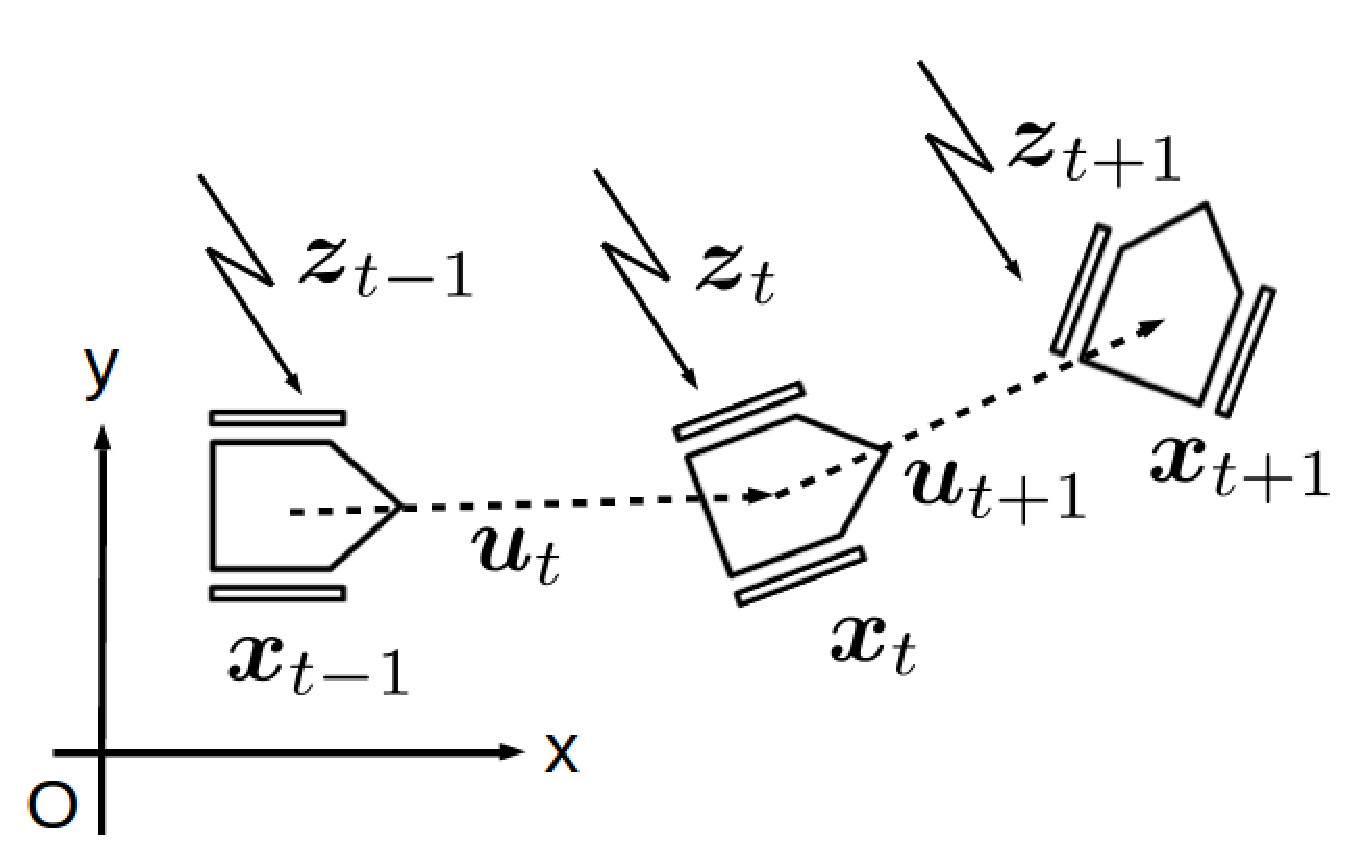
\includegraphics[width = 8cm]{./fig/symbol.eps}
        \caption{example of figure path}
        \label{fig::fig_path}
    \end{figure}
\end{verbatim}


\begin{figure}[htb]
    \centering
    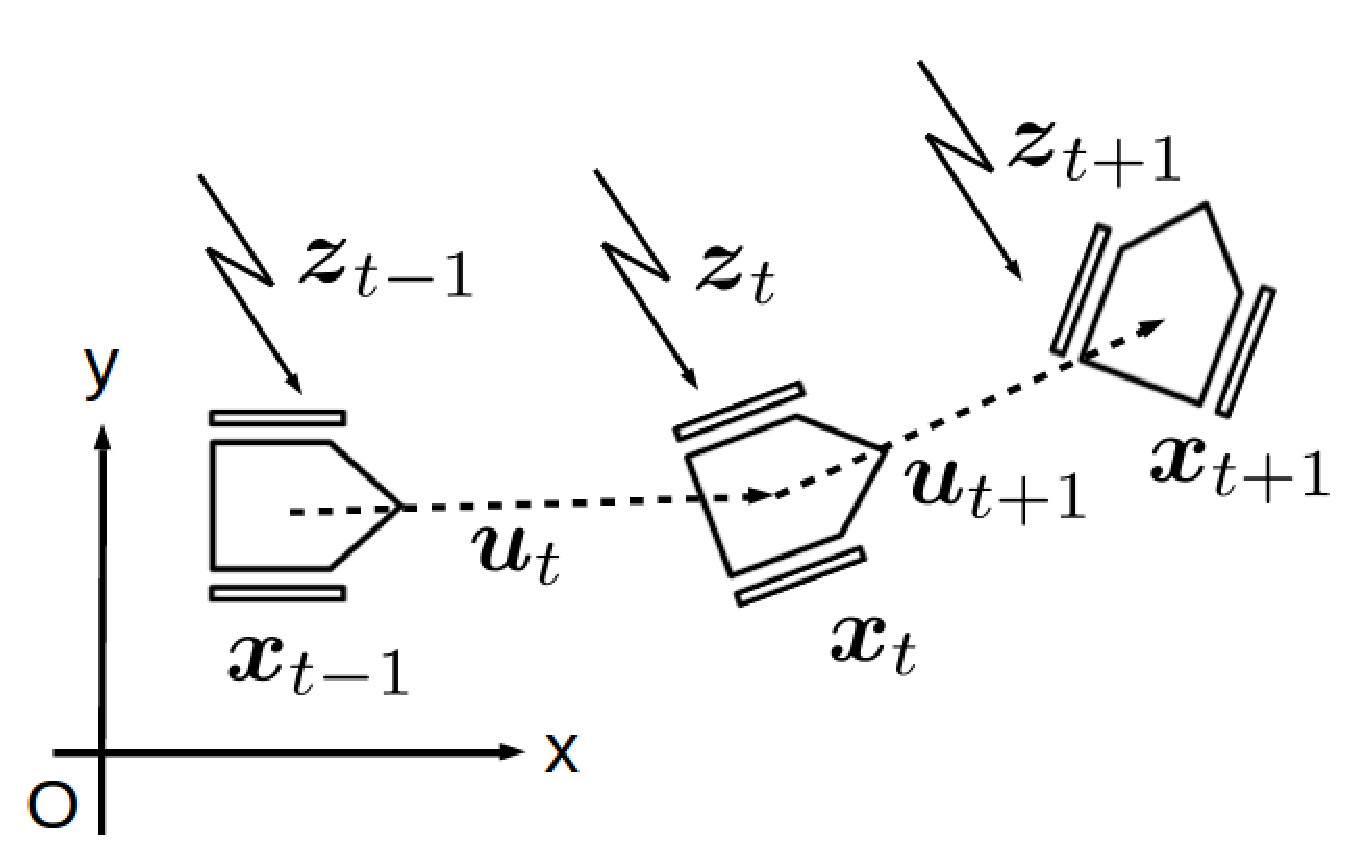
\includegraphics[width = 8cm]{./fig/symbol.eps}
    \caption{example of figure path}
    \label{fig::fig_path}
\end{figure}


% 参考文献リスト
\bibliographystyle{nya}
\bibliography{references}

% 付録
% % \small

\appendix
\chapter{amclのパラメータ}
\begin{verbatim}
    odom_model_type: diff
    odom_alpha5: 0.1
    transform_tolerance: 0.2
    gui_publish_rate: 10.0
    laser_max_beams: 30
    min_particles: 3000
    max_particles: 3000
    kld_err: 0.05
    kld_z: 0.99
    odom_alpha1: 0.2
    odom_alpha2: 0.2
    odom_alpha4: 0.4
    laser_z_hit: 0.5
    laser_z_short: 0.05
    laser_z_max: 0.05
    laser_z_rand: 0.5
    laser_sigma_hit: 0.2
    laser_lambda_short: 0.1
    laser_lambda_short: 0.1
    laser_model_type: likelihood_field
    laser_likelihood_max_dist: 2.0
    update_min_d: 0.2
    update_min_a: 0.5
    odom_frame_id: odom
    resample_interval: 1
    transform_tolerance: 0.1
    recovery_alpha_slow: 0.0
    recovery_alpha_fast: 0.0
\end{verbatim}

% \chapter{GNSS測位時のパラメータ}
% \begin{verbatim}
%     console-passwd     =admin
%     console-timetype   =gpst
%     console-soltype    =dms
%     console-solflag    =1
%     inpstr1-type       =serial
%     inpstr2-type       =tcpcli
%     inpstr3-type       =off
%     inpstr1-path       =sensors/gnss:115200:8:n:1:off
%     inpstr2-path       =133.232.64.13:5555
%     inpstr3-path       =
%     inpstr1-format     =ubx
%     inpstr2-format     =ubx
%     inpstr3-format     =rtcm3
%     inpstr2-nmeareq    =off
%     inpstr2-nmealat    =0
%     inpstr2-nmealon    =0
%     outstr1-type       =tcpsvr
%     outstr2-type       =off
%     outstr1-path       =localhost:52001
%     outstr2-path       =/home/hiroki/gnss_data/%Y%m%d%h%M.pos
%     outstr1-format     =llh
%     outstr2-format     =llh
%     logstr1-type       =off
%     logstr2-type       =off
%     logstr3-type       =off
%     logstr1-path       =rov_%Y%m%d%h%M.log
%     logstr2-path       =ref_%Y%m%d%h%M.log
%     logstr3-path       =8cor_%Y%m%d%h%M.log
%     misc-svrcycle      =10
%     misc-timeout       =3000
%     misc-reconnect     =3000
%     misc-nmeacycle     =5000
%     misc-buffsize      =32768
%     misc-navmsgsel     =rover
%     misc-startcmd      =./rtkstart.sh
%     misc-stopcmd       =./rtkshut.sh
%     file-cmdfile1      =../../../data/ubx_m8p_rov_bds_1hz.cmd
%     file-cmdfile2      =../../../data/oem4_raw_1hz.cmd
%     file-cmdfile3      =
%     pos1-posmode       =kinematic
%     pos1-frequency     =l1
%     pos1-soltype       =forward
%     pos1-elmask        =37
%
%     pos1-snrmask_ena1 = 1
%     pos1-snrmask_1_1 = 42
%     pos1-snrmask_1_2 = 42
%     pos1-snrmask_1_3 = 42
%     pos1-snrmask_1_4 = 42
%     pos1-snrmask_1_5 = 42
%     pos1-snrmask_1_6 = 42
%     pos1-snrmask_1_7 = 42
%     pos1-snrmask_1_8 = 42
%     pos1-snrmask_1_9 = 42
%
%     pos2-snrmask_ena2 = 2
%     pos2-snrmask_2_1 = 35
%     pos2-snrmask_2_2 = 35
%     pos2-snrmask_2_3 = 35
%     pos2-snrmask_2_4 = 35
%     pos2-snrmask_2_5 = 35
%     pos2-snrmask_2_6 = 35
%     pos2-snrmask_2_7 = 35
%     pos2-snrmask_2_8 = 35
%     pos2-snrmask_2_9 = 35
%     pos1-dynamics      =off
%     pos1-tidecorr      =off
%     pos1-ionoopt       =brdc
%     pos1-tropopt       =saas
%     pos1-sateph        =brdc
%     pos1-exclsats      =CO2
%     pos1-navsys        =63
%     pos2-armode        =fix-and-hold
%     pos2-gloarmode     =off
%     pos2-arthres       =3.0
%     pos2-arlockcnt     =0
%     pos2-arelmask      =0
%     pos2-aroutcnt      =5
%     pos2-arminfix      =0
%     pos2-slipthres     =0.05
%     pos2-maxage        =30
%     pos2-rejionno      =300
%     pos2-niter         =1
%     pos2-baselen       =0
%     pos2-basesig       =0
%     out-solformat      =llh
%     out-outhead        =on
%     out-outopt         =off
%     out-timesys        =gpst
%     out-timeform       =tow
%     out-timendec       =3
%     out-degform        =deg
%     out-fieldsep       =
%     out-height         =ellipsoidal
%     out-geoid          =internal
%     out-solstatic      =all
%     out-nmeaintv1      =0
%     out-nmeaintv2      =0
%     out-outstat        =off
%     stats-errratio     =100
%     stats-errphase     =0.3
%     stats-errphaseel   =0.3
%     stats-errphasebl   =0
%     stats-errdoppler   =1
%     stats-stdbias      =300
%     stats-stdiono      =0.03
%     stats-stdtrop      =0.03
%     stats-prnaccelh    =1
%     stats-prnaccelv    =1
%     stats-prnbias      =0.03
%     stats-prniono      =0.03
%     stats-prntrop      =0.03
%     stats-clkstab      =5e-12
%     ant1-postype       =llh
%     ant1-pos1          =0
%     ant1-pos2          =0
%     ant1-pos3          =0
%     ant1-anttype       =
%     ant1-antdele       =0
%     ant1-antdeln       =0
%     ant1-antdelu       =0
%     ant2-postype       =llh
%     #basestation
%
%
%     ant2-pos1          =36.111182791
%     ant2-pos2          =140.099188321
%     ant2-pos3          =92.1811          # (m|m)
%     ant2-anttype       =
%     ant2-antdele       =0          # (m)
%     ant2-antdeln       =0          # (m)
%     ant2-antdelu       =0          # (m)
%     misc-timeinterp    =off        # (0:off,1:on)
%     misc-sbasatsel     =0          # (0:all)
%     file-satantfile    =../../../data/igs05.atx
%     file-rcvantfile    =../../../data/igs05.atx
%     file-staposfile    =../../../data/station.pos
%     file-geoidfile     =
%     file-dcbfile       =../../../data/P1C1_ALL.DCB
%     file-tempdir       =../../../data/temp
%     file-geexefile     =
%     file-solstatfile   =
%     file-tracefile     =
% \end{verbatim}


\end{document}
